%-----------------------------------------------
% Dateiname: CreatePrototype.tex
% Autor    : Stefano Kowalke <blueduck@gmx.net>
% Lizenz   : BSD
%-----------------------------------------------
\section{Erstellung des Prototypen}
\label{prototype:sec:createPrototype}

\subsection{Die Grundstruktur}
Die Grundstruktur des Prototypen wurde unter \pdf{thesis/http/typo3conf/ext/doctrine\_dbal} erstellt.

\begin{Verbatim}[samepage=true]
.
└── doctrine_dbal/
    ├── Configuration/
    ├── Resources/
    ├── ext_emconf.php
    ├── ext_icon.gif
    └── ext_tables.php
\end{Verbatim}

Die Datei \pdf{ext\_emconf.php} enthält die Metainformationen der Extension, die vom Extension Manager verarbeitet werden.

\begin{listing}
\begin{phpcode}
<?php
$EM_CONF[$_EXTKEY] = array(
	'title' => 'Doctrine DBAL',
	'description' => 'Doctrine DBAL Integration in TYPO3 CMS',
	'category' => 'be',
	'author' => 'Stefano Kowalke',
	'author_email' => 'blueduck@gmx.net',
	'author_company' => 'Skyfillers GmbH',
	...
	'version' => '0.1.0',
	'constraints' => array(
		'depends' => array(
			'typo3' => '6.2.0-6.2.99',
		),
		'conflicts' => array('adodb', 'dbal'),
	...
	),
);
\end{phpcode}
\caption{Die Datei ext\_emconf.php}
\label{lst:extEmconf}
\end{listing}

Anschließend wurde Doctrine DBAL über \textit{Composer} installiert, indem es als externe Abhängigkeit in der \pdf{composer.json} definiert und durch das Kommando\\ \shinline{composer install} in den Ordner \pdf{vendor/doctrine} installiert wurde.

\begin{listing}[H]
\begin{jsoncode}
{
	"name": "typo3/doctrine_dbal",
	"type": "typo3-cms-extension",
	"description": "This brings Doctrine2 to TYPO3",
	"homepage": "http://typo3.org",
	"license": ["GPL-2.0+"],
	"version": "6.2.0",
	"require": {
		"doctrine/dbal": "dev-master"
	},
	"mininum-stability": "dev",
}
\end{jsoncode}
\caption{Die Datei composer.json}
\label{lst:composer}
\end{listing}


Die Integration von Doctrine DBAL sollte so transparent für TYPO3 CMS und die Extensions erfolgen, dass weiterhin über die Methoden der alten API auf die Datenbank zugegriffen werden kann. Die alte API steht dabei vergleichbar einer Fassade vor der neuen API, die ankommende Abfragen selbst behandelt oder an die neue API delegiert. Dieses Vorgehen erlaubt die sukzessive Integration von Doctrine DBAL.

Dazu wurde

\begin{itemize}
	\item im Ordner \pdf{doctrine\_dbal/Classes/Persistence/Doctrine} die Datei\\ \pdf{DatabaseConnection.php} erstellt (im weiteren Verlauf als \textit{neue API} bezeichnet),
	\item die Datei \pdf{DatabaseConnection.php} aus der Codebasis von TYPO3 CMS in den Ordner \pdf{doctrine\_dbal/Classes/Persistence/Legacy} des Prototypen kopiert (im weiteren Verlauf als \textit{alte API} bezeichnet),
	\item die Datei \pdf{DatabaseConnectionTests.php} aus der Codebasis von TYPO3 CMS in den Ordner \pdf{doctrine\_dbal/Tests/Persistence/Legacy} des Prototypen kopiert,
	\item eine Vererbung realisiert, die die Klasse der alten API von der Klasse der neuen API erben lässt (siehe Abb:.~\ref{fig:oldAPIextendsNewAPI})

\begin{figure}[H]
    \centering
    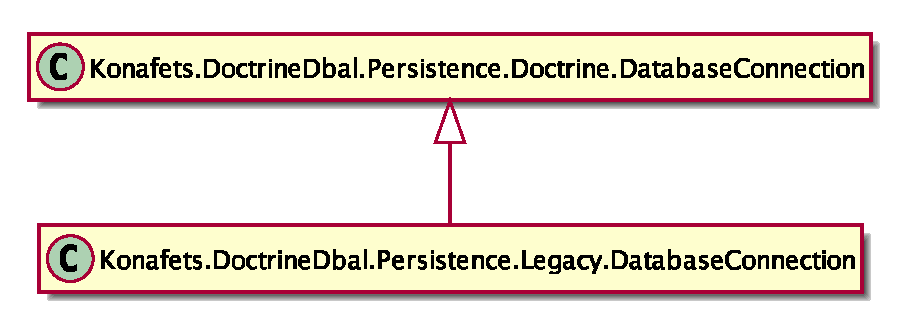
\includegraphics[scale=0.5]{gfx/uml/NewAPI/OldDatabaseConnectionExtentsFromNewAPI.eps}
    \caption{Alte API-Klasse erbt von neuer API-Klasse}
    \label{fig:oldAPIextendsNewAPI}
\end{figure}
	\item die Klasse der alten API per XCLASS in der Datei \pdf{ext\_localconf.php} registriert (Listing~\ref{lst:xclassDatabaseAPI}).
\end{itemize}


\begin{listing}[H]
\begin{phpcode}
if (!defined('TYPO3_MODE')) {
	die('Access denied.');
}

$GLOBALS['TYPO3_CONF_VARS']['SYS']['Objects']
  ['TYPO3\\CMS\\Core\\Database\\DatabaseConnection'] =
  array(
    'className'
      => 'Konafets\\DoctrineDbal\\Persistence\\Legacy\\DatabaseConnection'
  );
\end{phpcode}
\caption{Registrierung der XCLASSes in \pdf{doctrine\_dbal/ext\_localconf.php}}
\label{lst:xclassDatabaseAPI}
\end{listing}

Danach wurden alle Eigenschaften aus der alten API in die neue API verschoben und mit Setter/Getter-Methoden versehen, die von der alten API ab diesem Zeitpunkt genutzt wurden.

\subsection{Refactoring der alten API}
Die Umstellung auf Doctrine begann mit dem Refactoring der Methode \phpinline{connectDB()} der alten API. Dabei wurde lediglich die Implementation der Methode vereinfacht, da sie unübersichtlich war und mehrere unterschiedliche Aufgaben ausführte, die nichts mit deren Aufgabengebiet - der Herstellung einer Verbindung zur Datenbank - gemein hatten.

Neben ihrer eigentlichen Aufgabe hat sie

\begin{itemize}
	\item einen Test durchgeführt, ob eine Datenbank konfiguriert ist
	\item die konfigurierte Datenbank ausgewählt und
	\item verschiedene Hooks ausgeführt
\end{itemize}

Der Code, der nicht zur definierten Aufgabe der Methode gehörte, wurde in eigene Methoden ausgelagert. Die Methode zur Überprüfung der veralteten Parameter konnte gänzlich entfallen, da die Änderungen an der neuen API stattfanden. Die Methode wurde anhand des aufgestellten Namensschemas umbenannt und wird von der alten Methode aufgerufen. Zusätzlich fängt die Methode nun die von Doctrine DBAL kommende Exception wenn keine Verbindung erstellt werden konnte und wirft eine eigene \phpinline{ConnectionException}. Die entsprechenden Exceptionklassen wurden in\\ \pdf{doctrine\_dbal/Classes/Exeptions/} erstellt. Listing~\ref{lst:connectDatabaseAfterRefactoring} zeigt die Methode nach dem Refactoring; Listing~\ref{lst:connectDBcallsConnectDatabase()} zeigt den Aufruf der neuen Methode. Die originale Implementation der Methode ist in \pdf{typo3/sysext/core/Classes/Database/DatabaseConnection.php} ab Zeile 1578 zu finden.\footnote{\url{http://bit.ly/typo3cms-legacy-connectdb}}

\begin{listing}[H]
\begin{phpcode}
public function connectDatabase($isInitialInstallationInProgress = FALSE) {
	// Early return if connected already
	if ($this->isConnected) {
		return;
	}

	if (!$isInitialInstallationInProgress) {
		$this->checkDatabasePreconditions();
	}

	try {
		$this->link = $this->getConnection();
	} catch (\Exception $e) {
		throw new ConnectionException($e->getMessage());
	}

	$this->isConnected = $this->checkConnectivity();

	if (!$isInitialInstallationInProgress) {
		if ($this->isConnected) {
			$this->initCommandsAfterConnect();
			$this->selectDatabase();
		}

		$this->prepareHooks();
	}
}
\end{phpcode}
\caption{connectDatabase() nach dem Refactoring}
\label{lst:connectDatabaseAfterRefactoring}
\end{listing}

\begin{listing}[H]
\begin{phpcode}
public function connectDB(...) {
	...
	$this->connectDatabase();
}
\end{phpcode}
\caption{connectDB() delegiert an die neue API-Methode}
\label{lst:connectDBcallsConnectDatabase()}
\end{listing}

\subsection{Herstellen einer Verbindung}
Die Erstellung der Verbindung wurde in der alten API an die Methode \phpinline{sql_pconnect()} ausgelagert. \phpinline{getConnection()} ist der Name der Methode die diese Aufgabe in der neuen API übernimmt.

Zunächst wurde der Code, welcher nicht zum Aufgabengebiet der Methode gehört, in eigene Klassen ausgelagert. In dem Fall betraf das den Test nach einer installierten MySQLi PHP-Erweiterung, welcher im gleichen Zuge auf PDO geändert wurde. Die Initialisierung von Doctrine erfolgt in einer eigenen Methode. Dort wird je eine Instanz von \phpinline{\Doctrine\DBAL\Configuration} und \phpinline{\Doctrine\DBAL\Schema\Schema} erstellt. In der alten API bot die Methode die Möglichkeit einer persistenten Verbindung zur Datenbank. Dies wurde implementiert, indem ein eigenes \phpinline{PDO}-Objekt mit dem Konstrukturparameter \phpinline{\PDO::ATTR_PERSISTENT => true} erstellt und in dem Konfigurationsarray gespeichert wurde, welches im Anschluß an \phpinline{\Doctrine\DBAL\DriverManager::getConnection()} übergeben wurde (siehe Listing~\ref{lst:DoctrineConfigArray}).

\begin{listing}[H]
\begin{phpcode}
protected $connectionParams = array(
	'dbname'   => '',
	'user'     => '',
	'password' => '',
	'host'     => 'localhost',
	'driver'   => 'pdo_mysql',
	'port'     => 3306,
	'charset'  => 'utf8',
);
\end{phpcode}
\caption{Das Konfigurationsarray für Doctrine DBAL}
\label{lst:DoctrineConfigArray}
\end{listing}

Zudem muß Doctrine DBAL der Datentyp \sqlinline{Enum} bekannt gemacht werden. Anschließend wird der Schema Manager erstellt, welcher zur Verwaltung des Datenbankschemas notwendig ist. Am Schluß wird das Verbindungsobjekt zurückgegeben. Der Code ist in \phpinline{\Konafets\DoctrineDbal\Persistence\Doctrine\DatabaseConnect::getConnection()}\footnote{\url{http://bit.ly/1sOXU1q}} zu finden.

\subsection{Implementation der grundlegenden Methoden}
Nachdem durch Doctrine DBAL die Verbindung hergestellt werden konnte, wurde die Methode \phpinline{query()} der alten API übernommen. Sie stellt die zentrale Schnittstelle aller API-Methoden zum Senden ihrer Abfragen an die Datenbank dar. Sie kapselt die gleichnamige Methode \phpinline{\Doctrine\DBAL\Connection::query()}.

\newpage

\begin{listing}
\begin{phpcode}
protected function query($query) {
	if (!$this->isConnected) {
		$this->connectDatabase();
	}

	$stmt = $this->link->query($query);

	return $stmt;
}
\end{phpcode}
\caption{getConnection() der neuen API}
\label{lst:getConnectionNewAPI}
\end{listing}

Wie bereits in Kapitel~\ref{basics:doctrine:subsubsec:simpleDatabaseQueries} erwähnt wurde, gibt \phpinline{query()} ein Statementobjekt zurück, welches die Ergebnismenge bereithält. Dort wurde ebenfalls dargestellt, dass diese Menge durch die Methode \phpinline{fetch()} in Verbindung mit PDO-Konstanten in Index-basierte oder Assoziative Arrays formatiert werden kann.

Um die Arbeit mit der Ergebnismenge zu erleichtern wurden die drei Methoden\\ \phpinline{fetchAssoc($stmt)}, \phpinline{fetchRow($stmt)} und \phpinline{$fetchColumn($stmt)} implementiert, die die am häufigsten vorkommenden  \textit{Fetch-Styles} kapseln.

\begin{phpcode}
public function fetchAssoc($stmt) {
	if ($this->debugCheckRecordset($stmt)) {
		return $stmt->fetch(\PDO::FETCH_ASSOC);
	} else {
		return FALSE;
	}
}
\end{phpcode}

Die ehemaligen \phpinline{admin_*}-Methoden wurden in \phpinline{list_*}-Methoden umbenannt, da die Unterscheidung in Admin und Nicht-Admin Methoden nicht nachvollziehbar war. Diese Methoden stellen wichtige Metainformation zur darunterliegenden Datenbank bereit, die nicht nur für das \textit{Install Tool} von Nutzen sind.

Als Beispiel der Abstraktion, die Doctrine DBAL mitbringt, sei die Implementation der Methode \phpinline{listDatabases()} angeführt. Nach dem obligatorischen Verbindungstest, gibt der \phpinline{SchemaManager} eine Liste aller Datenbanken zurück - vollkommen unabhängig von der zugrundeliegenden \gls{dbms}.

\begin{phpcode}
public function listDatabases() {
	...
	$databases = $this->schemaManager->listDatabases();
    ...
	return $databases;
}
\end{phpcode}

Im Gegensatz zur alten API, dessen Methode ein Backslash (\phpinline{\}) den zu maskierenden Zeichen voranstellt, werden die Zeichen von Doctrine durch ein Hochkomma (\phpinline{'}) maskiert. Die Methode \phpinline{\Doctrine\DBAL\Connection::quote()} wurde in der neuen API durch eine gleichnamige Methode gekapselt und stellt die Basis für alle weiteren Methoden wie \phpinline{fullQuoteString()}, \phpinline{fullQuoteArray()}, \phpinline{quoteString()} und \phpinline{escapeStringForLike()} dar, welche das Verhalten der alten Methoden implementieren.

Die neue API bietet dagegen die Methoden \phpinline{quoteColumn()}, \phpinline{quoteTable()} und\\ \phpinline{quoteIdentifier()} zum Maskieren an. Sicherer ist jedoch von Anfang die Benutzung von Prepared Statements, welche von TYPO3 CMS seit Version 6.2 in Form eines Wrappers um die Prepared Statements von MySQLi angeboten werden. Sie besitzen die gleichen API, wie sie in Kapitel~\ref{basics:doctrine:subsubsec:preparedStatements} vorgestellt wurden.

Durch den Aufruf der Methode \phpinline{$stmt = $GLOBALS['TYPO3_DB']->prepare($sql)} wird zunächst das Objekt vom Typ \phpinline{\TYPO3\CMS\Core\Database\PreparedStatement} erstellt, dem der in \phpinline{$sql} gespeicherte Prepared Statement übergeben wird. Ein Aufruf von\\ \phpinline{$stmt->bind(':lastName', 'Potter')} fügt einem internen Array des Objekts diese Werte hinzu. Zusätzlich wird versucht den Datentyp zu erkennen und ebenfalls zu speichern. Erst mit dem Aufruf von \phpinline{$stmt->execute()} wird die Datenbank kontaktiert. Zuvor wird jedoch erst die gespeicherte SQL-Abfrage und - die durch \phpinline{bind()} - übergebenen Parameter von \textit{Named Placeholder} in \textit{Positional Parameter} transformiert, da MySQLi nur diese unterstützt. Daraufhin wird die SQL-Abfrage über \phpinline{mysqli::prepare()} an die Datenbank gesendet. Danach werden die in dem Array gespeicherten  Parameter per \phpinline{mysqli::bind()} an die Abfrage gebunden und abschließend per \phpinline{mysqli::execute()} ausgeführt. Zur Definition des Datentypes und des \textit{Fetch-Styles} werden Konstanten wie \phpinline{PreparedStatement::PARAM_INT} oder \phpinline{PreparedStatement::FETCH_ASSOC} verwendet.

Zur Umstellung auf Doctrine wurde die Datei \pdf{PreparedStatement.php} TYPO3 CMS nach \pdf{doctrine\_dbal/Classes/Persistence/Doctrine/} kopiert. Es wurden die eigens verwendeten Konstanten auf PDO-Konstanten umgemappt und die Transformation in \textit{Positional Parameter} wurde entfernt, Doctrine DBAL beide Varianten unterstützt.

\begin{phpcode}
protected function guessValueType($value) {
	if (is_bool($value)) {
		$type = PDO::PARAM_BOOL;
	} elseif (is_int($value)) {
		$type = PDO::PARAM_INT;
	} elseif (is_null($value)) {
		$type = PDO::PARAM_NULL;
	} else {
		$type = PDO::PARAM_STR;
	}

	return $type;
}
\end{phpcode}
